\section{Appendix: implementation details}
\label{app:impl}

\paragraph{Scoring pass.}
For every expression we store: the released semantic score under four text
variants (full expression, spatial-stripped, content-only, head noun phrase),
the negative-noun score, the released GEM coherence score, per-proposal mask
area, centroid and bounding box, the strict-containment parent of every
proposal, the pool pairwise IoU matrix, and the per-proposal IoU against
ground truth (the union of the reference's masks on gRefCOCO). Everything
else in this paper is a re-analysis of these records; the records themselves
come from one forward pass per dataset
(\texttt{exp/exp4\_guided\_full.py}, \texttt{exp/exp21\_grefcoco\_full.py}).

\paragraph{Shipped configuration.}
Candidate base $=$ rank$(S^{\mathrm{dec}})+\gamma\,$rank$(S^{\mathrm{coh}})$
with $\gamma=0.49$; $k=15$; overlap mode $=$ IoU; selection $=$ argmax of the
mode over the candidates; growth off. These five values are the best of
\studyTrials{} Optuna trials on the held-out split, objective $=$ minimum over
datasets of mIoU (\texttt{exp/out\_final/optuna\_study\_sent.json}); the
noun-phrase study is the second file. The earlier repairs (relation-gated
operator with $k=8$ and a two-axis gate, containment growth at
$|A\cap B|/|A|\ge0.95$) are reported as ablations and are off in the shipped
configuration.

\paragraph{Bounding-box prior.}
Prompt: ``Locate the \{expression\} in this image. Reply with ONLY the
bounding box as [x0,y0,x1,y1] in pixel coordinates measured from the
top-left corner, or the single word none if it does not appear in the
image.'', with the full expression substituted. Decoding is greedy,
\texttt{max\_new\_tokens}{}$=32$; the reply is parsed for its first four
numbers and values $\le1.5$ are read as normalised coordinates. Boxes are
cached per (image, expression) under \texttt{exp/out\_vlm\_boxes/}; the
vision tower pass is cached per image. The 8-bit backend
(\texttt{exp/convert\_llavaov\_hf.py} converts the cached checkpoint to the
HF layout so the standard bitsandbytes path applies) produced the same boxes
as bf16 on our agreement sample.

\paragraph{GRES extension.}
Clause split on top-level ``and''/``or''/``,''; one box per clause; per-clause
selection by Eq.~\ref{eq:select}; union of the selected masks; empty output
when every clause answers \texttt{none}.

\paragraph{Compute.}
All scoring passes ran on 4$\times$RTX~4090. Per dataset the pass costs
about 0.9--1.2 GPU-hours; the entire paper (four datasets, plus controls and
ablations, which are CPU re-analyses) is under 6 GPU-hours.

\paragraph{Val-pass ledger and reproduction pins.}
Every arm in the learned-prior table and the transfer-inversion study is a
single frozen application of the full official val split. Within the
transfer-inversion study that is five new configurations (recipe,
recipe$+$combination policy, strata-$\{1,2\}$, weights-only, tau-only), seven
pre-registered leave-one-rare-ref-out refits (diagnostics only; the shipped
row was declared unchanged on any outcome), and two bit-reproduction passes
for the cluster bootstrap; the weak-signal democracy probe ran on a seeded
$800$-row val sample under its own single-pick protocol (its number is a
sample mIoU, never a full-val cIoU). Arm, threshold and weight selection used
the held-out train carve-out only. Reproducing the shipped recipe bit-exactly
requires \texttt{OMP\_NUM\_THREADS=4} (as the shipped runs used): under a
different thread count the logistic-regression fits drift in the last decimal,
two margin-boundary rows flip their rank-1 second part, and the train table
rebuilds with $10{,}352$ parts instead of $10{,}351$ (val $52.684$ vs
$52.706$); under the pin an independent control refit reproduces the shipped
row exactly.

\section{Appendix: per-dataset detail}
\label{app:detail}

\paragraph{Taxonomy per dataset.}
Table~\ref{tab:taxonomy} reports the oracle-gap taxonomy on all four
benchmarks; the wrong-instance share is stable across datasets and across two
scorers that differ by ~10 mIoU.

\paragraph{Strata and quartiles.}
On RefCOCO val the operator's gain decomposes by relation type: horizontal
$n=\strataHorizontalN$ \strataHorizontalD, vertical $n=\strataVerticalN$
\strataVerticalD, middle $n=\strataMiddleN$ \strataMiddleD, ordinal
(abstains) and no-relation (abstains) zero by construction. By ground-truth
area quartile the operator is positive in all four
(\oursQOne\,/\,\oursQTwo\,/\,\oursQThree\,/\,\oursQFour), while the growth
control's gain is confined to the largest.

\paragraph{gRefCOCO rows.}
Table~\ref{tab:gres} lists every row of the gRefCOCO evaluation, including
the margin sweep for plural expansion and the two controls (no relation
gate, no growth).

\paragraph{Published-number transcription.}
Published rows in Table~\ref{tab:sota} were transcribed from the GLOD-RIS
Table~I and HybridGL Table~1 PDFs (both in the repository under
\texttt{papers/}) and cross-checked between the two sources where they
overlap.


\section{Appendix: qualitative examples}
\label{app:qual}

\begin{figure*}[t]\centering
\ifx\undefined\IfFileExists\else\fi
\IfFileExists{figures/qualitative.pdf}{%
  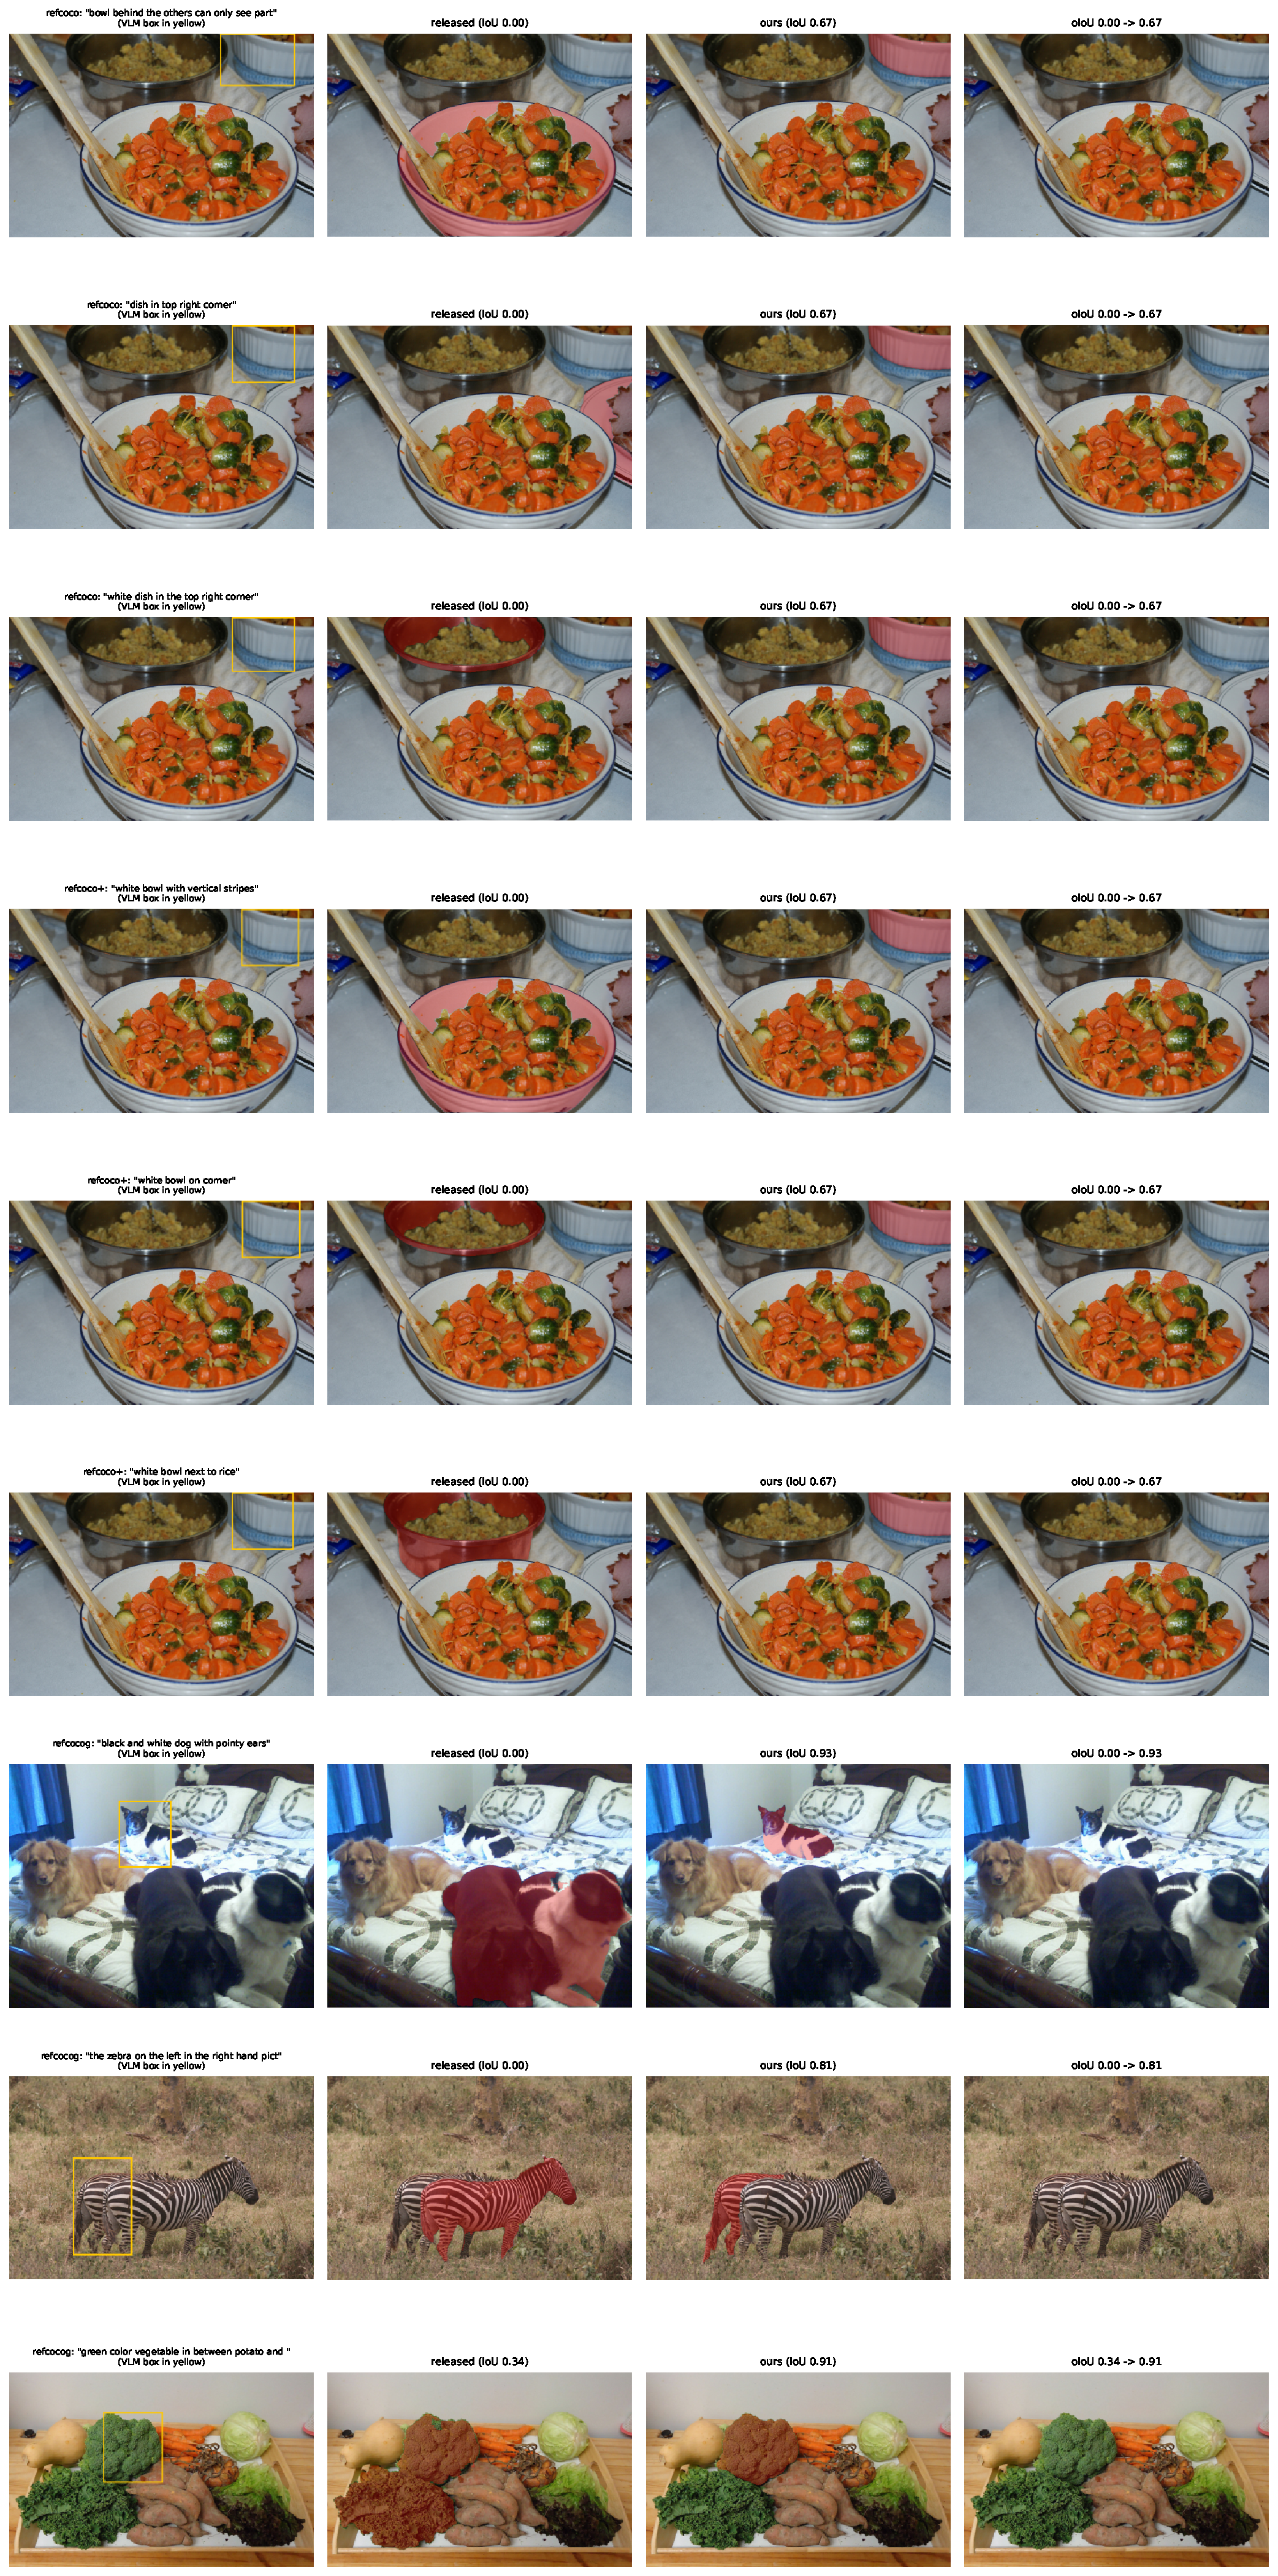
\includegraphics[height=0.90\textheight,keepaspectratio]{figures/qualitative.pdf}%
}{%
  \fbox{\parbox{0.9\textwidth}{\centering qualitative panel pending (exp/exp45\_qualitative.py)}}%
}
\caption{Examples where the box prior changes the selection (one per dataset
family, selected by a criterion fixed in \texttt{exp/exp45\_qualitative.py}:
the method and the released pipeline disagree and the IoU gap exceeds $0.25$).
Column 1 shows the VLM box (yellow) overlaid on the image and the expression;
columns 2--3 the released selection and ours. Ground-truth IoU is in each
title. These are illustrative, not a random sample.}
\label{fig:qual}
\end{figure*}

\section{Appendix: evidence map}
\label{app:evidence}

Every claim in the paper maps to a stored artifact:
\texttt{exp/out\_final/main\_\{refcoco,refcocoplus,refcocog,grefcoco\}.json}
(one per dataset; all rows, CIs, strata, quartiles, taxonomy);
\texttt{exp/out\_final/gref\_topk\_reselection.json} and
\texttt{gref\_learned\_selector\_transfer.json} (change 16 and the documented
negative transfer result);
\texttt{exp/out\_final/protocol\_audit.json} (the metric-protocol audit of
\S\ref{sec:protocol}: per-dataset protocol source, metric definition, and the
re-evaluation of the saved predictions under it, with the numbers after
alignment --- including the completed gRefCOCO coverage and the pooled oIoU);
\texttt{exp/out\_final/ablation.json} (each row with its own evidence file);
\texttt{exp/out\_final/sota\_table.json} (measured rows carry evidence paths;
published rows carry transcription sources);
\texttt{refine-logs/METHOD\_GRAVEYARD.md} (killed methods and the control
that killed each);
\texttt{paper/figures/specs/architecture.json} and the rendered
\texttt{architecture.pdf} (deterministic vector figure);
\texttt{exp/out\_extreme/records\_*.jsonl} (the scoring passes every analysis
reads);
\texttt{exp/out\_final/headroom.json} (the structural cause: top-3
containment, oracle rank, category-score top-8);
\texttt{exp/out\_final/cross\_dataset.json} (the dose-response and the
residual strata);
\texttt{exp/out\_final/pool\_robustness.json} (points-per-side 8 vs 16);
\texttt{exp/out\_final/evidence/repro\_blocks.json} with the raw logs
\texttt{repro\_official\_blockA.log} and \texttt{repro\_official\_blockB.log}
(the two disjoint reproduction-audit blocks);
\texttt{exp/out\_final/optuna\_study\_\{noun,sent\}.json} (the two
\studyTrials{}-trial studies and their per-dataset held-out mIoU);
\texttt{exp/tuning/*\_refs.json} (the held-out split: seeded train refs);
\texttt{exp/out\_vlm\_boxes/} (one cached VLM box per expression);
\texttt{exp/out\_final/gref\_ceiling.json} (the gRefCOCO no-target wall:
oracle set-IoU, the leaky logistic bound, and the $\mathrm{N\text{-}acc}$
requirement at perfect masks);
\texttt{exp/out\_final/exp37\_\{refcoco,refcocog\}\_gt.json} and
\texttt{exp37\_vlm\_sample800.json} (the box-prior ceiling and its
realistic-box sample);
\texttt{exp/out\_final/optuna\_study\_gref\{2,3,4,5\}.json} (the gRefCOCO
held-out studies: hand rules, learned selector, decision rules, clause
features; \studyTrials{} trials each);
\texttt{exp/out\_final/gref\_exists\_probe\_sh*.json} and the
\texttt{exists} cache namespace (the single yes/no presence probe);
\texttt{exp/out\_final/gref\_ensemble\_\{roc,val\}.json},
\texttt{gref\_rule\_showdown.json}, and
\texttt{gref\_ensemble\_aggregates.json} (the three-prompt presence ensemble:
held-out rule selection, full-val frontier, and the exact union-mass
requirements behind the shipped row);
\texttt{exp/out\_final/gref\_wall.json} (the three-axis wall analysis and the
exact oracle-realization requirement);
\texttt{exp/out\_final/gref\_tuned\_val2000.json} and
\texttt{exp/out\_final/gref\_full\_val.json} (the frozen gRefCOCO model's
validation evaluation).
